\documentclass[border=4pt]{standalone}

\usepackage{tikz}

\definecolor{otblue}{HTML}{0072B2}
\definecolor{otorange}{HTML}{E69F00}
\definecolor{otteal}{HTML}{009E73}
\definecolor{otpurple}{HTML}{CC79A7}
\definecolor{otgray}{HTML}{5A5A5A}

\begin{document}
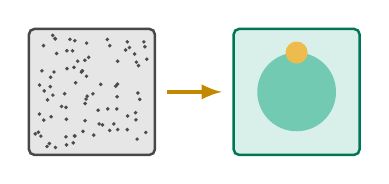
\begin{tikzpicture}[line width=0.9pt]
  \pgfmathsetseed{7}
  \filldraw[draw=otgray!80!black, fill=otgray!15, rounded corners=2pt] (0,0) rectangle (1.6,1.6);
  \foreach \i in {1,...,85}{\fill[otgray!85!black] ({0.08+1.44*rnd},{0.08+1.44*rnd}) circle[radius=0.025];}
  \draw[otorange!85!black, line width=1.5pt, -latex] (1.75,0.8) -- (2.45,0.8);
  \filldraw[draw=otteal!75!black, fill=otteal!15, rounded corners=2pt] (2.6,0) rectangle (4.2,1.6);
  \fill[otteal!55] (3.4,0.8) circle[radius=0.5];
  \fill[otorange!70] (3.4,1.3) circle[radius=0.14];
\end{tikzpicture}
\end{document}
